\documentclass{article}
\usepackage{amsthm, amssymb, latexsym, amsmath, amsbsy, graphicx, epsfig}
\usepackage{ mathrsfs }
\usepackage{ textcomp }
\usepackage{titling}
\usepackage[top=1in, left=1.2in, right=1.2in, bottom=1.2in]{geometry}
\usepackage{tocloft}
\usepackage{caption}
\usepackage{ragged2e}
\usepackage{fancyhdr}
\graphicspath{{figures/}}


\fancyhf{}
\pagestyle{fancy}
\fancyhead[L]{\raggedright MTH-240 : Allocca}
\fancyhead[R]{\parbox{6cm}{\centering \raggedleft  \leftmark}}  
\pagenumbering{roman} 
\setcounter{page}{1} 
\setlength{\headsep}{50pt} 
\setlength{\cftbeforesecskip}{0pt}
\setlength{\cftbeforesubsecskip}{-6pt} 
\renewcommand{\baselinestretch}{2} 
\fontsize{12}{13.5}\selectfont
\setlength{\parskip}{1em} 
\setlength{\parindent}{0pt} 
\title{\textbf{MTH-240: Transitions to Abstract Mathematics  Proof Portfolio}}
\author{$\mathbb{R}$obert T Kohn}
\date{$\forall$pril 30th  2025}
\begin{document}
\maketitle
\begin{center}
\vspace{-3.033em}
\noindent\rule{0.7\linewidth}{0.5pt}

\

\textbf{Claim: If the Mets won the world series, then I am Mickey Mouse.}
\end{center}
Let P = ``Mets win the world series" $\wedge$ Q = ``I am Mickey Mouse" $\ni  \ P \Rightarrow Q$

Then, P is false

Thus, $P \Rightarrow Q$ is true

$\therefore$ I am Mickey Mouse. \boxed{Q.E.D} //

\begin{flushright}
\textit{``If you use ergo, then you just sound like a complete asshole"} 

\vspace{-2em}
-Allocca, Michael. The Art of The Proof
\end{flushright}



\newpage
\tableofcontents

\

\vspace{0.5cm}
\begin{center}
    \fbox{\parbox{0.8\textwidth}{\centering \large \textbf{How to Read This Document:} \\
    This document is divided into several sections, each of which explores a different topic within this course. \\
    Where each subsection for every topic is the proof referenced in that section. \\
    Each section summarizes the contents and findings of the proofs while expresing the revisions that took place and the greater knowledge gained by the proof.\\
    I hope you find this piece enjoyable and remember to be skeptical when it comes to math!}}
\end{center}

\newpage
\fancyhf{}
\pagestyle{fancy}
\fancyfoot[L]{Kohn}
\fancyfoot[R]{\thepage} 
\fancyhead[L]{\raggedright MTH-240 : Allocca}
\fancyhead[R]{\parbox{6cm}{\centering \raggedleft MY PERSONAL REFLECTION AND GROWTH}}  
\pagenumbering{arabic}
\setcounter{page}{1} 
\section*{My Personal Reflection and Growth over the Semester}
\addcontentsline{toc}{section}{My Personal Reflection and Growth over the Semester}
\subsection*{Acknowledgments}
\addcontentsline{toc}{subsection}{Acknowledgments}
\begin{center}
\justifying
This course has been a challenging but deeply rewarding journey. As a student, I have drastically increased my ability to construct logical arguments, moving from intuition to structured proofs, as well as becoming proficient in LaTeX, a tool I now consider indispensable. I am excited to see what I am capable of with LaTeX going forward as it is a powerful tool with academic writing and also it can be reformatted fairly easily. The built in nature of editing equations and writing them is super convenient and has a lot of potential. I also anticipate using LaTeX in my future in my CUEs and also as a teacher. I want to have that perfectly typeset font I have been fortunate to use in all my courses at Muhlenberg thus far. LaTeX is a career asset I am fortunate to have learned. It will also be a nice tool to present on resumes, some may even be typeset in it. Beyond just the importance of LaTeX, I have learned how to effectively use propositional logic, quantifiers, induction, direct and indirect proving methods while also developing a clearer understanding of sets, families, relations, partitions, and function. This course has been monumental to my development as a Math, Physics, and Statistics major. Coming from a family with a heavy legal background, this course was fascinating and I understand why you recommend this course to upcoming lawyers.

\end{center}

\subsection*{How the Concept of Mathematical Proof has Changed Over the Semester}
\addcontentsline{toc}{subsection}{How the Concept of Mathematical Proof has Changed Over the Semester}

\begin{center}
\justifying
Coming into this course, I couldn't tell you what a real proof was. I likely would have told you its akin to proving a theorem but I wouldn't be able to tell you how. I probably would have been like dot dot dot, see the pattern? If I had to write even the most basic of proofs, I'm sure I would laugh at myself looking back. We started light talking about case by case examples as well as working with truth tables to validate tautologies and case analysis but slowly we upped the ante. We began to work with quantifiers and induction and slowly my logic went from intuition to highly academic reasoning. I think one of the most important realizations which occurred during this course was the concept of inverses, converses, and contrapositions and how they hold up versus the original claim. That was mind blowing for me at first. Furthermore, the journey of proving with examples and isolated steps to connected reasoning is something which shouldn't be overlooked so easily. This was a process which was developed through practice and demonstration in class. Within this course as well, mathematical proofs went from being algebraic and linear to being abstract and modular which are concepts I likely couldn't consider coming into this course. In the end, this course transformed the idea of what it means to prove something, not only as a process but as a rigorous and logical way of thinking.
\end{center}


\subsection*{What Improved and What Needs Growth}
\addcontentsline{toc}{subsection}{What Improved and What Needs Growth}

\begin{center}
\justifying
In the last passage, I wrote about how fundamentally speaking my concept of what proving is and just how it is done and what it means has changed me. There has been so much growth in this course, likewise there has been much stagnation. Starting with the good, I am a much more confident proof writer and can combine complex ideas with precision. However, despite understanding these complexities, I have fallen short with my prose countless times even within my latest assignments. There have even been times where my proof writing style has been so clunky that it has resulted in getting the wrong point across or explaining something poorly. Stagnation in this category is fatal if I wish to develop strong proofs. Often times, I've failed to realize the true error within proofs and have even falsely assumed some true proofs were actually false. Despite all these chronic issues,  I have a very concise and powerful proof writing style. With time and more careful revisions, I believe that I can become an even stronger proof writer than I am now. I look to Real Analysis and possibly Abstract Algebra with joy and excitement.

\end{center}
\newpage
\fancyhf{}
\pagestyle{fancy}
\fancyfoot[L]{Kohn}
\fancyfoot[R]{\thepage} 
\fancyhead[L]{\raggedright MTH-240 : Allocca}
\fancyhead[R]{\parbox{6cm}{\centering \raggedleft  \leftmark}}  
\section{Direct Proof}
\justifying
The first proof comes from Section 1.6 on Question 1E and is focused around a direct proof. In comparison to the original, within this version of the proof, I declared variables very early on and tightened the prose to simplify the overall proof. As far as direct assumptions go, it starts with the clear assumption that t=15m+16n and assumes the truth of the statement. It follows tight logical steps to reach the conclusion as it defines the new variables in terms of the previous ones and algebraically manipulates it while maintaining the defined relationships. Further, it doesn't use any indirect reasoning such as contraposition or contradiction. Therefore, it follows the format of a direct proof as it assumes, shows that it follows, and that it applies for all scenarios.

\subsection{$(\forall t \in \mathbb{Z}), (\exists m,n \in \mathbb{Z}) \ni 15m+16n=t  \Rightarrow  (\exists r,s \in \mathbb{Z}) \ni 3r+8s=t$ }
\begin{center}
\raggedright
Suppose 15m+16n=t and r=5m and s=2n:

Then,  3r+8s=3(5m)+8(2n)=15m+16n=t

 $\therefore (\exists r,s \in \mathbb{Z}) 3r+8s=t $ \boxed{Q.E.D} //

\end{center}
\newpage
\section{Indirect Proof}
\justifying
As for the indirect proof, it is best to look at Section 2.1 on Question 7. In the original, I felt as if I formatted it poorly in LaTex and so I improved it by adding some bold face and cleaning up extraneous details I felt were poor. I attempted to be more clear in my assumptions and their implications as well. I also made sure to explicitly state the logic used to reach that conclusion rather than hoping my reader infers. This proof is strong as an indirect proof and is specifically a proof by contradiction as it assumes the opposite and then shows the logical contradiction which forces the original to be true. First and foremost, it directly states that I am negating the conclusion, that is to say that the hypothesis is true and the conclusion is false. By using a definition logically, it leads to a contradiction where x is both $\in$ and $\notin$ B which is impossible(unless it's Schrödinger's element or something silly). This results in concluding that inconsistency can only be avoided by accepting the original implications of the claim. It is a very simple logical structure which relies on key definitions and allows for the logical collapse with contradiction and indirect proofs.
\newpage
\subsection{$x\notin B \wedge A \subseteq B \Rightarrow x \notin A$}
\
\begin{center}
\raggedright
\textbf{Suppose Not}

[WTS: Contradiction x's relationship with B]

Suppose $x\notin B \wedge A \subseteq B \wedge x\in A \ $:

Then,  $x \in A \wedge A \subseteq B \Rightarrow x \in B$.

Thus, this contradicts the assumption that $x \notin B$, when $x\in A $

$\therefore x\notin B \wedge A \subseteq B \Rightarrow x \notin A$ \boxed{Q.E.D} //

\end{center}
\newpage
\section{Proof with Quantifiers}
\justifying
The following proof is one that I truly enjoyed doing and was really the eye opener for me with proofs. It comes in Section 1.4 on Question 1E. I really liked this proof because it establishes the principles of odd and even numbers which is simple to someone who understands any math and it's almost like a ``oh duh" moment with every proof yet it's the principle that informs our past knowledge of these facts. This serves as an elementary basis for number theory but it applies to complex properties of numbers too. It also seems very easy to just want to divide off rip or create fractions or anything else besides prove by factoring. It's one of those proofs which were challenging to grasp early on but make complete logical sense now that I've taken this whole course and it was a pleasure to rewrite in that regard. Now with respect to how this applies to quantifiers. From the start of the proof, the proof asserts that there exists some integers k and c that make up x and y. This is the fundamental fact of how existential quantifiers work as they simply claim there exists. Such indications imply that not all k and c work, however, there is at least one which makes it work. It also helps clarify the scope of the problem as it makes x and y mean something rather than just being odd. It allows for further assumptions be made with m and it's summation to an even number.
\begin{center}
\fbox{\parbox{0.8\textwidth}{\centering\textbf{\large{Proof}}

Let \( P(x) \) be "Person \( x \) loves pizza."

Suppose \( \exists x \ \ni \neg P(x) \)

This is a contradiction as pizza is amazing.

$\therefore$ \( \forall x  \in \, P(x) \), everyone loves pizza. \(\boxed{\text{Q.E.D.}} //\)}}
\end{center}

\newpage
\subsection{x is odd $\wedge$ y is odd $\Rightarrow x+y$ is even}
\
\begin{center}
\raggedright
Suppose $(x, y \in \mathbb{Z}) \ni$ x and y are both odd.

Then, $(\exists c, k  \in \mathbb{Z}) \ni x=2k+1 \wedge y=2c+1$

[WTS: $(\exists m  \in \mathbb{Z}) \ni x+y=2m$]

Thus, x+y=2k+2c+2=2(k+c+1)

Hence, $(\exists m  \in \mathbb{Z}) \ni x+y=2m$

$\therefore$ x+y is even \boxed{Q.E.D} //

\end{center}

\newpage
\section{Multi-Step Proof}
\justifying
One of my favorite Multi-Step Proofs was within Section 2.2 on Question 9B. It's a pretty simple set problem but has some pretty fun implications and includes multiple unique steps. I started the proof with proof by contradiction which allows for a multi-step reasoning pattern. I then analyze the contradicting implications within this new claim within set containment and the realization that elimination infers $x \in B$. From there it connects to the logical contradiction within the conditions and concludes that the original implication is true because of the contradiction. This whole proof highlights the interactions of unions, intersections, and subset relations. This proof can also be applied to data processing and memory retrieval in coding. This proof serves as a framework to filter multiple sources and access memory quickly in code.

\newpage
\subsection{$A \subseteq B \cup C \wedge A \cap B = \emptyset \Rightarrow A \subseteq C$}
\
\begin{center}
\raggedright
\textbf{Suppose Not}

Suppose:  $A \subseteq B \cup C \wedge A \cap B = \emptyset \wedge A \nsubseteq C$

Then, $(\exists x\in A) \ni x \notin C$

[WTS: $x \in A \cap B \wedge A \cap B=\emptyset$]

Thus, $x\in B \cup C$

So, $x \in B$

Hence, $x \in A \cap B$

But, there is a contradiction because $A \cap B = \emptyset$

$\therefore A \subseteq B \cup C \wedge A \cap B = \emptyset \Rightarrow A \subseteq C$ \boxed{Q.E.D} //


\end{center}

\newpage
\section{Proof by the Principle of Mathematical Induction}
\justifying
I really enjoyed induction and the next proof comes from Section 2.4 on Question 5C. I wanted to make a conscious effort with this one to be clearer and concise while explaining the logical connections between each part of the proof while achieving mathematical precision with consistent terminology. This proof itself is particularly interesting as it gives an interesting look at cubic expressions as it connects algebraic expressions with divisibility rules. As a PMI problem, it does everything very cut and dry I felt. It has to follow a classic inductive reasoning process from the base case to the inductive step. The inductive hypothesis is algebraically manipulated in such a way that allows for k+1 to become divisible by 6. It efficiently uses PMI to reach the conclusion and so I thought it would be a perfect example.

\begin{center}
\fbox{\parbox{0.8\textwidth}{\centering\textbf{\large{I'm always early to MTH-240 because of MTH-227}}\\

\textbf{Base Case - Suppose: 1st day:}

I was in MTH-240 early because of MTH-227

\textbf{Inductive Hypothesis - Suppose: k-th day:} 

Assume I was early because of MTH-227 on the k-th day

\textbf{Inductive Step - Suppose: k+1 day}

I will be early on the \( k+1 \)-th day, because, I always have MTH-227.

$\therefore$ I'm always early to MTH-240 because of MTH-227 \(\boxed{\text{Q.E.D.}} //\)}}
\end{center}

\newpage
\subsection{$n^3-n$ is divisible by 6}
\
\begin{center}
\raggedright
\textbf{Base Case - Suppose n=1:}

Then, $1^3-1=0$

\textbf{Inductive Hypothesis - Suppose: n=k}

$(\exists a,k \in \mathbb{Z}) \ni k^3-k=6a$

\textbf{Inductive Step - Suppose: n=k+1}

Thus, $(k+1)^3-(k+1)=k^3+3k^2+2k=(k^3-k)+3k^2+3k$

So, using the inductive hypothesis, $6a+3k^2+3k=6a+3k(k+1)$

Hence, k(k+1) is always even since the product of two consecutive numbers is even

Then, $(\exists b \in \mathbb{Z}) \ni (k+1)^3-(k+1)=6a+6b=6(a+b)$

$\therefore$ By PMI, $n^3-n$ is divisible by 6 for all n  \boxed{Q.E.D} //
\end{center}

\newpage
\section{Proof by the Principle of Complete Induction}
\justifying
Building on the idea of induction, the Principle of Complete Induction is easily one of the most interesting things we have covered in this course. Section 2.5 offers an interesting example on Question 1. It offers an early insight on integer partitions and their combinations but I get more in depth on this within Section 13. Another application of this is when looking at resource allocation for fixed quantities which is something frequently viewed within Calculus optimization problems. It can also be related to dynamic programming where the computer solves problems by breaking them down into smaller problems and then stores them for future use. The big question is how does this proof differ from Proof by Mathematical Induction beyond just showing more base cases? They follow similar logical principles but don't have the same process or solution style. Proof by Mathematical Induction works on the premise that it works for the base case and then some arbitrary k and also when k+1. In contrast, Proof by Complete Induction highlights that it works for all n up to a certain value and then uses those previous values to prove that n+1 works. This is typically more useful when a problem uses recursion. In this problem, PMI would assume that the case holds for some k directly but PCI allows for stronger inductive practice. PCI shows that it holds for all values 23 to n and then uses n+1 which is more efficient within this problem's structure because it builds on previous values.
\newpage

\subsection{$(\forall \ n>22 \in N) (\exists s, t \in Z) \ \ni \ n=3s+4t \wedge s \geq 3 \wedge t \geq 2$}
\
\begin{center}
\raggedright
Case n=23: $\ni$ s=5, t=2

$3(5)+4(2)=15+8=23$

Case n=24: $\ni$ s=4, t=3

$3(4)+4(3)=12+12=24$

Case n=25: $\ni$ s=3, t=4

$3(3)+4(4)=9+16=25$

Hence, this statement holds for n=23, 24, and 25

Then, $(\exists k \in \mathbb{Z}) \ni 23 \leq k \leq n \wedge n \geq 25$ 

Thus,  $(\exists s, t, \mathbb{Z}) \ni s \geq 3 \wedge t \geq 2 \wedge k=3s+4t$

So, $n+1=(n-2)+3$

Hence, $n-2 \geq  23 \Rightarrow n+1=3s+4t+3$

Then, $n+1=3(s+1)+4t$

Thus, $(\exists s' \ni s'=s+1 \geq 4) n+1=3s'+4t'$

$\therefore$ By PCI, $(\forall \ n>22 \in N) (\exists s, t \in Z) \ \in \ n=3s+4t \wedge s \geq 3 \wedge t \geq 2$ \boxed{Q.E.D} //


\end{center}

\newpage
\section{Concise Proof}
\justifying
The concise proof I want to focus on is really simple and can be found in Section 1.6 on Question 4B. When I originally did this proof, I didn't even understand how to properly format a proof and had to revise it as a result. This one isn't overly complex as it simply establishes that if something is added to a negative version of itself then it's zero. Nothing shocking to be found here but it was easily the most concise proof as one could argue that the reader could infer the result from the suppose line alone. However, for clarity's sake we connect the dots for them in proofs. This proof although easy now built the foundation for quantifiers and the idea of the additive inverse while holding for all numbers.

\subsection{$ \forall x \exists y (x+y=0) $}
\
\begin{center}
\raggedright

Suppose $\exists x \in \mathbb{R} \ni y=-x$

Then, x+y=x+(-x)=0

$\therefore \forall x \exists y (x+y=0) $\boxed{Q.E.D} //
\end{center}



\newpage
\section{Chapter 1 Proof}
\justifying
I find that I enjoy proofs most when they are connected to something super complex that we are aware of and Section 1.6 Question 3 really exemplifies this. For starters, the proof is based entirely around an unproven conjecture with the boogie man prize which was never claimed. It also questions the very existence of number theory as it questions if 1 is a prime number. If 1 is a prime number it breaks everything but also solves many things so that is very fun to think about. The proof starts by assuming something which is unproven in the Goldbach Conjecture which I find super fun because it's technically illogical but also must be done for the whole claim to have any relevance beyond just a truth table example. This proof is also interesting as one would presume that as there are odd numbers greater than 5 it should be increasingly harder to decompose into sums of primes but the proof showcases this to be an incorrect line of logic. This proof also lays early groundwork with regards to more in depth mathematical induction techniques done down the line as it starts with small cases like odd numbers greater than 5. This proof also takes extremely complex ideas like parity and breaking it down into simple components to make it easy to solve. This proof obviously showcases basic proof methods but to elaborate it assumes the antecedent(Goldbach Conjecture) and builds on that assumption. It also uses universal and existential quantifiers establishing further usage of Chapter 1 material. It also looks into number theory as it explores the complexities of Goldbach's Conjecture and expands it into a new argument involving odd and prime numbers.


\newpage

\subsection{Goldbach Conjecture 2.0}
\
\begin{center}
\raggedright
Suppose $(\forall n>2 \in \mathbb{N} \ni$ n is even) n is the sum of two primes:

Let $n>5 \in \mathbb{N}$ be an odd number and $\mathbb{P}$ be the universe of prime numbers.

[WTS: n-1=2m to use Goldbach Conjecture]

Then, $(\exists m \in \mathbb{ N}) n=2m+1>5$

Thus, n-1=2m $\Rightarrow$ n-1 is even

So, by the assumption that every even number greater than 2 is the sum of two primes, n-1 can be expressed as the sum of two primes $\Rightarrow n-1=p_1+p_2 \ni (p_1 \wedge p_2 \in \mathbb{P}$)

Hence, $n=p_1+p_2+1$

$\therefore$ Every odd number greater than 5 is the sum of 3 prime numbers \boxed{Q.E.D} //
\end{center}
\newpage
\section{Chapter 2 Proof}
\justifying
I feel like no proof better encapsulated the nature of Chapter 2 than Section 2.3 Question 14. It tackles the concept of set theory as it deals with pairwise disjoint sets where their intersection is empty. This is fundamental when it comes to understanding the relationships in chapter 2. It also involves set operations as it refers specifically to the idea of intersection with pairwise disjoint and also highlights the empty set and intersection. Further, this problem is based on the idea of indexed family sets. It claims that \( \mathcal{A} \) is a family of pairwise disjoint sets and claims \( \mathcal{B} \) is the same. It unfortunately doesn't include true induction or counting but it could theoretically be applied to calculate the total number of distinct elements in each family. This proof is overall very interesting as it covers a lot of mathematical ground. It also has connections to future class endeavors such as partitioning.

\begin{center}

\fbox{\parbox{0.8\textwidth}{\centering\textbf{\large{All Proof Writers are Unique.}}\\

Let \( P_1, P_2, \dots, P_n \) be an indexed family of Dr. Allocca's MTH-240 Students. 

Then, Since they are pairwise disjoint, no two of them have anything in common, including their proof structure.

$\therefore$ All proof writers are unique \(\boxed{\text{Q.E.D.}} //\)}}

\end{center}

\newpage
\subsection{\( \mathcal{A} \) is a family of pairwise disjoint sets. \( \mathcal{B} \subseteq \mathcal{A} \) $\Rightarrow$ \( \mathcal{B} \) is a family of pairwise disjoint sets}
\
\begin{center}
\raggedright
Suppose \( \mathcal{A} \) is a family of pairwise disjoint sets $\wedge$  \( \mathcal{B} \subseteq \mathcal{A} \):

[WTS: \( \mathcal{B} \) is a family of pairwise disjoint sets.]

Then, for any two distinct sets $\left( X,Y \right)$  $\in$ \( \mathcal{B} \) $\Rightarrow \left( X \right)\wedge \left( Y \right) \in$ \( \mathcal{A} \)

Thus, $ X \neq Y \Rightarrow X \cap Y = \emptyset$

Hence, as X and Y are arbitrary, this holds for any sets in \( \mathcal{B} \)

$\therefore$  \( \mathcal{B} \) is a family of pairwise disjoint sets. \boxed{Q.E.D} //
\end{center}
\newpage
\section{Chapter 3 Proof}
\justifying
The thing I enjoyed most from Chapter 3 was easily the way relations work, this proof comes from Section 3.2 on Question 17. First and foremost, the following proof leverages symmetry and transitive relations to deduce reflexivity which really highlights the way all 3 are interrelated. Even though we are not given reflexivity, we can infer it based on the others. However, all of this only works through the power of composition and building on top of the foundations of other parts. Understanding the assumption within the domain is also crucial when solving a proof like this as it guarantees we are working within set A and that all elements within A are in play. Relations are thought to be subsets of the cartesian pairs and the operations on them are directly linked with things like intersections and unions and it brings everything together neatly. This proof allows for further generalizations as well as showcases their fundamental relations. This proof doesn't specifically highlight partitions or modular arithmetic but it does have comparable elements to what occurs in the proof.

\begin{center}

\fbox{\parbox{0.8\textwidth}{\centering\textbf{\large{Wegmans Turkey is the Best.}}\\

Let \( T_w \) be Wegmans turkey $\wedge$ \( T_g \) be turkey from the local grocery store $\wedge$ \( T_d \) be turkey from the deli. 

Then, $T_w > T_g  \wedge  T_g > T_d$

By the transitive property, \( T_w > T_d \)

$\therefore$ Wegmans turkey is the best.  \(\boxed{\text{Q.E.D.}} //\)}}

\end{center}

\newpage
\subsection{R is symmetric and transitive relation on A $\wedge$  Dom(R)=A $\Rightarrow$ R is reflexive on A.}
\
\begin{center}
\raggedright
Suppose: R is symmetric and transitive relation on A $\wedge Dom(R)=A$

Then, $(\exists a,b \in A) \ni (a,b) \in R$

So, $(a,b) \in R \Rightarrow (b,a) \in R$ by symmetry

Hence, $(a,b) \in R \wedge (b,a) \in R \Rightarrow (a,a) \in R$

$\therefore$ R is reflexive on A. \boxed{Q.E.D} //
\end{center}
\newpage
\section{Chapter 4 Proof}
\justifying
The proof I elected to go with for our latest endeavor into functions and disproving and delving into what we know about them takes place in Section 4.3 on Question 5B. I liked this proof a lot as I felt it brought a lot of complex topics together. This proof works with functions as relations as it treats it as a set of ordered pairs and its reflection of how functions are really just subsets of cartesian products. This proof is focused around explicit constructions of functions, in this case within the modular arithmetic domain $\mathbb{Z}_4$ to $\mathbb{Z}_2$. This proof also highlights the full concept of bijectivity as it breaks up surjectivity and injectivity during the proof and evaluates accordingly. Further, this proof works with set images within modular arithmetic. The analysis of these image sets are a key application of the concept. This proof specifically is very interesting as it focuses on surjectivity without injectivity. Many functions we have studied historically have been true bijections or broken. Additionally, this proof can be related to linear transformations within vector spaces like in linear algebra.

\begin{center}

\fbox{\parbox{0.8\textwidth}{\centering\textbf{\large{The Mets always have a winning pair.}}\\

Let \( (x, y) \) be an ordered pair $\ni$ \( x \) is the Mets’ pitcher $\wedge$ \( y \) is their batter. 

Then, one of them is always throwing the game $\wedge$ the other is always striking out.

$\therefore$ The Mets are doomed to be in sports purgatory \(\boxed{\text{Q.E.D.}} //\)}}

\end{center}


\newpage
\subsection{$f: \mathbb{Z}_4 \rightarrow \mathbb{Z}_2$ given by $f(\overline{x})=[3x]$ is onto but not one to one.}
\
\begin{center}
\raggedright
Evaluating:

$f(\overline{0})=[0]=[0]$

$f(\overline{1})=[3]=[1]$

$f(\overline{2})=[6]=[0]$

$ f(\overline{3})=[9]=[1]$

Onto:

Then, the image of f is $\{[0], [1]\}=\mathbb{Z}_2$

Thus, every element of the codomain has a preimage.

So,  f is onto.

Not one to one:

Then, $f(\overline{0})=f(\overline{2})=[0]$

So, f  distinct elements yield the same output.

Hence, f is not one to one.

$\therefore f: \mathbb{Z}_4 \rightarrow \mathbb{Z}_2$ given by $f(\overline{x})=[3x]$ is onto but not one to one. \boxed{Q.E.D} //
\end{center}

\newpage
\section{Proof which Needed Revision}
\justifying
The proof which needed revision for me came within Writing Assignment \#8 and takes place within Section 3.1 on Question 11B. In the original proof I tried supposing the contrapositive. This was a fundamentally sound proof but didn't guarantee the existence of such an x existing in the first place for Dom(S \textopenbullet R). After revising initially, I realized I needed to include that (y,z) is within S as well in order to complete the pairing. This proof is fundamentally interesting as it plays a massive role in how query optimization and a lot of database referencing works. But when it comes to mathematics, it focuses on set theory and the way the domain of composed relations is limited by the domain of the inner relation. This proof also makes use of implications and existential quantifiers the whole way through.

\newpage
\subsection{Dom(S \textopenbullet R) $\subseteq$ Dom(R)}
\
\begin{center}
\raggedright
Suppose $x \in$ Dom(S \textopenbullet R)

Then, $\exists z \ni (x,z) \in $ (S \textopenbullet R)

Thus, $\exists y \ni (x,y) \in R \wedge (y,z) \in S$

So, $x \in $ Dom(R)

$\therefore$ Dom(S \textopenbullet R) $\subseteq$ Dom(R) \boxed{Q.E.D} //

\end{center}
\newpage
\section{Proof That I Found Interesting}
\justifying
The following proof takes place in Section 2.5 on Question 1C. When looking at it for the first time, it is a relatively challenging run of the mill proof by complete induction problem. However, when applying it to recent developments in our course, it is clear that it is applicable to what we learned more recently with partitions. This proof establishes the idea that after 33, all natural numbers are able to be combined by some non-negative integer combination of fours and fives which is pretty fascinating to think about. It sounds extremely strange to think about and say out loud but makes perfectly logical sense. This type of logic is something which I also explored in a side project I did for Darin Thomas in the weight room. He had the question of how many possible combinations you could possibly do for 50 pull ups which led me to learning about partitions early and something far too advanced for my full understanding in the Euler Recurrence Formula. The principle is established in this proof and has lots of value when expanded upon. Further, this proof was extremely fun to work with and challenging in its own right. It starts as a small observation with algebraic observations but leads to sophisticated results and reasoning. I loved this proof and I'm fortunate enough to present it as the one I found most interesting.
\newpage
\subsection{ $(\forall \ n>33 \in \mathbb{N}) (\exists s, t \in \mathbb{Z}) \ \ni \ n=4s+5t \wedge s \geq 3 \wedge t \geq 2$}
\
\begin{center}
\raggedright
$Case \ n=34: \ \ni  s=6, t=2$

$4(6)+5(2)=24+10=34$

$Case \ n=35: \ \ni s=5, t=3$

$4(5)+5(3)=20+15=35$

$Case \ \ n=36: \ \ni s=4, t=4$

$4(4)+5(4)=16+20=36$

$Case \ n=37: \ \ni s=3, t=5$

$4(3)+5(5)=12+25=37$

Suppose $\exists n \geq 34 \wedge n=4s+5t \wedge s \geq 3 \wedge t \geq 2$:

Then, $n+1=(n-4)+5$

Thus, $n-4=4s+5t \Rightarrow n+1=4s+5t+5$

So, $n+1=4s+5t+5 \Rightarrow n+1=4s+5(t+1)$

Hence, $(\exists t' \ni t'=t+1 \geq 3) n+1=4s+5t'$

$\therefore (\forall \ n>33 \in \mathbb{N}) (\exists s, t \in \mathbb{Z}) \ \ni \ n=4s+5t \wedge s \geq 3 \wedge t \geq 2$ \boxed{Q.E.D} //

\end{center}

\newpage
\section{A Fun Biconditional and Set Theory Proof}
\justifying
The next proof is focused around biconditionality and set theory and takes place in Section 2.2 on Question 19B.  It focuses on if and only if statements which are logically type and works to show that for any x it holds. It takes the fundamentals of set operation, union, intersection, and set difference, in a way which allows for a complex combination of these ideas for an advanced conclusion. Biconditionality is also super important as something we've practiced because it allows the proof to go fully both ways. When revising this proof I was trying to consider the advice that I had gotten wrong in both submissions which was the jump of logic at the end. In this final rendition, I understood I must more deliberately seperate where and when x is in or out of A and B. 
\newpage

\subsection{$A \Delta B = (A \cup B) - (A \cap B)$}
\
\begin{center}
\raggedright
 $\exists x \in U \ni $ U is the universal set.

$x \in A \Delta B \leftrightarrow x \in (A-B) \cup (B-A)$

[WTS: $x \in  (A \cup B) \wedge x \notin (A \cap B)$]

$ \leftrightarrow (x \in A \wedge x \notin B) \vee (x \notin A \wedge x \in B)$ 

$ \leftrightarrow (x \in A \vee x \in B) \wedge ~(x \in A \wedge x \in B)$ 

$\leftrightarrow x \in  (A \cup B) \wedge x \notin (A \cap B)$

$\leftrightarrow x \in  ((A \cup B) - (A \cap B))$

$\therefore  A \Delta B = (A \cup B) - (A \cap B)$ \boxed{Q.E.D} //
\end{center}

\newpage
\section{Alden Handshake Problem}
\justifying
Oh goodness, where to start with this problem. This proof originates from an assignment given with lots of restrictions and theoreticals on how many handshakes Mr. Alden's wife shook at this strange party where you must track how many hands you shook. Quite silly but very interesting and complex. There are lots of unique interactions while also considering the involvement of induction and real world applications that made me so excited. My brain couldn't process this all at first and I overthought it to the point where it was necessary to try and map it out visually. Eventually after so much trial and error, I realized that there had to be zero hand shakes and that otherwise the model breaks. Then after further failures of modeling, I realized that there must be a power couple and that Mrs. Alden always happened to land in the middle. From there I started thinking about how to apply my realizations to the real proof and it kind of fell into place like a bunch of legos. I wrote it so poorly the first time I probably nearly sent Dr. Allocca into cardiac arrest. However, I properly approached induction this time and not only that but I neatened it up. This whole problem really resulted in a bunch of ranked ordered pairs which I find so fascinating to see how it all comes together. This problem, on top of reinforcing other mathematical principles, also reinforces the way we can apply our logic skills to more than just math. Overall, this was the highlight of the course for me I think, such a fun project with lots of creative freedoms.

\begin{figure}[h]
\

    \centering
    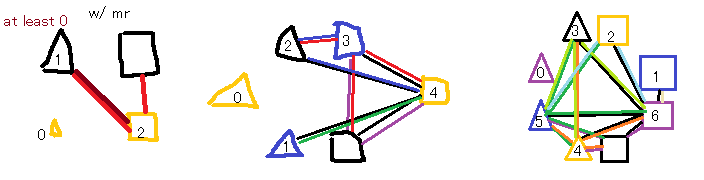
\includegraphics[width=0.9\textwidth]{alden_handshake_model.png}
    \caption*{Aforementioned Drawn Model of the Handshakes for $n\leq2$}
\end{figure}



\newpage

\subsection{Mrs. Alden shook n hands, where n is the number of other couples at the party}
\raggedright
Let n denote the number of other couples at the party.

{\textbf{Base Case - Suppose n=1:}}

Then, the Aldens and 1 other couple are at the party $\Rightarrow$ there is 3 people whose handshake count matters. 

Since, each person Mr. Alden asked has a unique hand shake count then those besides Mr. Alden could only have shook 0 hands, 1 hand, or 2 hands.

Thus, one partner must have shook the Alden's hands while their partner shook neither.

So, Mrs. Alden must have shook one hand because she can't shake her husband's hand.

{\textbf{Inductive Hypothesis - Suppose $\exists k \geq 1$, n=k:}}

Then, Mrs. Alden shook k hands.

{\textbf{Inductive Step - Suppose n=k+1}}

Since the Alden's are a married couple, they cannot shake each others hands, and cannot become the power couple.

Hence, the new couple has distinct and maximized handshake behaviors $\ni$ they are the power couple. 

[WTS: Mrs. Alden shakes k+1 hands $\vee$ There are 2k+2 possible handshakes.]

Then, the Alden's have k+1 other couples at the party $\Rightarrow$ there are 2k+3 people whose handshake count matters.

Thus, there are 2k+2 maximum possible handshakes because there is one person within the power couple who shakes no hands.

So,  Mrs. Alden must shake k+1 hands.

$\therefore$ Each person has a unique hand shake count $\wedge$ no one shook their own hand $\wedge$ no partners shook hands $\wedge$ no two people shook hands more than once $\wedge$ there are $n \geq 1$ other couples at the party $\Rightarrow$ Mrs. Alden shook n hands, where n is the number of other couples at the party. \boxed{Q.E.D} //

\begin{center}
     \fbox{\parbox{1\textwidth}{\centering \Huge \textbf{Quod Erat Demonstrandum} \\
    \huge Which was to be demonstrated. \\
    \large Cheers to another great semester and course! Have a great summer, thank you for reading my proof portfolio, and putting up with my nonsense!}}



\includegraphics[width=0.45\textwidth]{muhlenberg_mule.png}


\includegraphics[width=0.4\textwidth]{muhlenberg_berg.png}


\end{center}



\end{document}
